\section{Rust Embedded Library}

This section describes the library facilities provided by Rust that are usable in an barebone embedded setting.
From considering the dependencies for \textbf{std} in Figure \ref{fig:rust:librust} we see that this crate is not suitable for a barebones application.
The dependency on either an Unix or Windows OS excludes \textbf{std} and all its dependents from being used without an OS.
The remaining Rust Embedded Library, REL, is shown in Figure \ref{fig:rust:rel}.

\begin{figure}[H]
  \begin{center}
    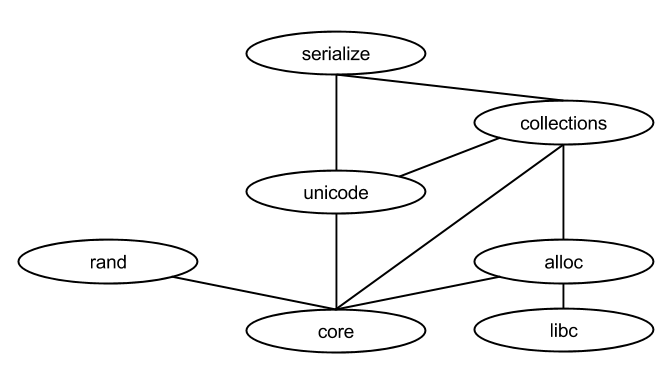
\includegraphics[scale=0.3]{figures/background/rust/embedded-rust-lib.png}
  \end{center}
  \caption{Rust Embedded Library, REL}
  \label{fig:rust:rel}
\end{figure}

The remainder of this section examines the contents of the different crate composed into REL.

\subsection{Rust Core Library}

The Rust Core Library, RCL, defines the platform independent non-dependent core of the Rust language.
For normal usage the Rust Standard Library, RSL, augments RCL with platform dependent features and reexports the stable parts.
In this way RCL is not interfaced with directly and can modified as long as the interface though RSL stays the same.
With REL the programmer must interface with RCL directly.

REL mainly defines the primitive types of Rust and operations on these in addition to memory management and some core language traits.

\subsubsection{Primitive types}

Table \ref{tab:rust:datatypes} lists the primitive datatypes available in Rust.
RCL defines functions for manipulating these datatypes.

\begin{table}[H]
  \begin{tabular}{l|l}
    array & fixed-length array type \\
    bool & data type with value true or false \\
    char & a unicode scalar value \\
    f32, f64 & floating point number of single and double precision \\
    i8, i16, i32, i64, u8, u16, u32, u64 & integers \\
    isize, usize & integers of 'pointer-sized' size \\
    pointer & raw unsafe pointers (*const T, *mut T) \\
    slice & a view into a array \\
    str & string \\
    tuple & finite ordered list of elements
  \end{tabular}

  \caption{Primitive datatypes}
  \label{tab:rust:datatypes}
\end{table}

Most of the datatypes in Table \ref{tab:rust:datatypes} brings no surprises with the when it comes to representation and functionality.
The ones who are not common place are discussed in below.

\paragraph{Pointer}

Rust exposes a few different pointer types.
Within RCL is a raw pointer type.
This pointer is not generally used in Rust code and is considered unsafe.
These pointers are used for interfacing with C code and writing data structure not permitted by safe pointers. \todo{Should probably show the restrictions related to doubly-linked lists}

\paragraph{Slice}

The slice type is simply a view into an array.
The representation is a pointer and a length as shown in Listing \ref{lst:rust:slice}.

\begin{listing}[H]
  \begin{minted}{rust}
    pub struct Slice<T> {
      pub data: *const T,
      pub len: usize
    }
\end{minted}
\caption{Slice representation}
\label{lst:rust:slice}
\end{listing}

Slices have special syntax denoted by \&[T] where T is a type.

\paragraph{str}
\label{par:rust:str}

The Rust string type str can either be a statically allocated string defined as a literal or a borrowed reference into another string.
A string in Rust is a sequence of Unicode scalar values and is not null terminated.
The representation of the string type is closely related to slices as \&str is equivalent to \&[u8].

\paragraph{tuple}

A tuple type is a fixed size datatype of variable types.
The type can be used to return multiple return values from a function.
In addition the type supports tags just like the variants of an enum.

\subsubsection{Memory Management}
\subsubsection{Core Language Traits}

\subsection{Allocation}
\label{sec:rust:allocation}

The RCL does not use or expose any heap allocation.
Heap allocation is introduced through the \texttt{Box} type defined in the allocation library.

\subsection{The Collection Library}

The Rust collection library provides the data structures shown in Table \ref{tab:rust:collections}.

\begin{table}[H]
  \begin{tabular}{l}
    Binary Heap \\
    Binary Tree Map \\
    Binary Tree Set \\
    Bit Set \\
    Bit Vector \\
    Enum Set \\
    Linked List \\
    Vector \\
    Vector Dequeue \\
    Vector Map \\
    String \\
  \end{tabular}
  \caption{Rust Collection Library}
  \label{tab:rust:collections}
\end{table}

We look at some of the data structures in this section.

\subsubsection{Vector}

The Vector is an important data structure both in direct usage but also as a building block for other data structures.
In essence it is a growable heap allocated list of values of the same type.

\subsubsection{String}

In section \ref{par:rust:str} we discussed the \textbf{string slice}.
The \texttt{String} defined in the collection library is a heap allocated mutable string.

\subsection{libc}

The heap allocation library described in Section \ref{sec:rust:allocation} depends on the \texttt{libc} crate abstraction.
The \texttt{libc} library provided in the standard library provides bindings for the C standard library and platform specific libraries.
REL depends on \texttt{libc} for the low level memory operations \texttt{malloc}, \texttt{realloc} and \texttt{free}.
The details of this implementation is found in Section \ref{sec:impl:libc}. \todo{Update reference to implementation chapter part about libc implementation}

\subsection{Notable missing functionality in REL}

- Reference Counted GC
